\documentclass[11pt, oneside]{article}
\usepackage[margin=1in]{geometry}
\geometry{letterpaper}
\usepackage{booktabs}
\usepackage{hyperref}
\usepackage{enumitem}
\usepackage{float}
\usepackage{caption}
\usepackage{subcaption}
\usepackage[numbers]{natbib}
\usepackage{graphicx}
\usepackage{amssymb}
\usepackage{amsmath}
\usepackage{array}
\usepackage{longtable}
\usepackage{xcolor}
\usepackage{tabularx}
\usepackage{setspace}
\usepackage{tikz}
\usetikzlibrary{shapes.geometric,arrows.meta,positioning,fit,backgrounds,calc}
\definecolor{slate}{RGB}{112,128,144}
\hypersetup{
    colorlinks=true,
    linkcolor=blue,
    citecolor=blue,
    urlcolor=blue
}
% ============================================================
% TITLE BLOCK --- students must keep this format
% Replace placeholders. Do not redesign the title page.
% Filename of the compiled PDF must be:
% CS781-CP-[Firstname]-[Lastname]-[RollNo]-report.pdf
% ============================================================
\title{CS781 Capstone Project:\\
In-House Legal Intelligence System}
\author{
    Shubham Joshi \\
    240500 \\
    {\tt shubhamj24@iitk.ac.in}\\
    Indian Institute of Technology Kanpur (IIT Kanpur)
}
\date{}
\setlength{\emergencystretch}{2em}
\begin{document}
\maketitle

\begin{abstract}
This project builds a self-hosted legal NLP system from four compact models pretrained
on the official legal corpus using a custom byte-level tokenizer. Their descendants
cover entity extraction, rhetorical roles, judgment prediction, statutes, summaries
and case retrieval. Full fine-tuning, low-rank adaptation, adapters, prompts and
distillation provide task-specific solutions within dual-T4 compute limits.
Resumable training, exact span alignment and hierarchical document encoding support
reliable execution. Best reported results include 0.7705 judgment Macro-F1,
0.8353 summarization BERTScore and 0.4365 retrieval Micro-F1@7. The experiments
demonstrate the value of compact legal representations, careful adaptation and
task-specific inference.
\end{abstract}

\section{Competition Result}
\noindent\textbf{Codabench username:} \texttt{s\_240500}\hfill\textbf{Roll number:} 240500
\begin{table}[H]\centering\small
\caption{Best reported competition results and ranks, supplied on 9 November 2026.
Metric 1 and Metric 2 retain the supplied result-column labels.}
\label{tab:leaderboard}
\setlength{\tabcolsep}{4pt}
\begin{tabular}{clrrrrr}\toprule
Phase & Task & Score & Rank & Submissions & Metric 1 & Metric 2\\\midrule
1 & Legal LM & 0.8348 & 38 & 4 & 0.1928 & 0.0546 \\
2 & Legal NER & 0.4851 & 89 & 7 & 0.5304 & 0.4636 \\
3 & Rhetorical roles & 0.4560 & 93 & 6 & 0.5114 & 0.4853 \\
4 & Judgment prediction & 0.7705 & 31 & 6 & 0.7867 & 0.7454 \\
5 & Statute identification & 0.3970 & 41 & 6 & 0.4878 & 0.0517 \\
6 & Summarization & 0.8353 & 81 & 6 & 0.4335 & 0.2096 \\
7 & Case retrieval & 0.4365 & 46 & 11 & 0.4454 & 0.4279 \\
\bottomrule\end{tabular}\end{table}
\noindent\textbf{Public repository:} \url{https://github.com/SHUB-1806/CS781_capstone}.\\
\textbf{Total valid submissions:} 46 (author-confirmed counts: 4, 7, 6, 6, 6, 6, 11).
The per-phase counts meet the report template's four-submission minimum. The source
bundle includes the selected model for each phase, configurations, data preparation,
evaluation and reproducibility instructions. Submission IDs, filenames and supplied
submission timestamps are recorded in \texttt{code/competition\_results.csv}.

\section{Introduction and Problem Description}
Legal documents contain sensitive facts, long arguments and precise references to
people, courts and statutes. A self-hosted system can keep document processing within
institutional infrastructure. This project studies that setting under a restricted
training corpus, a 50M--300M foundation-parameter budget and Kaggle GPU resources.
The goal was to build the pipeline from pretraining through task adaptation, without
importing an external pretrained task model or using an external generation API.

Phase 1 predicts a 128-word continuation from a 512-word prompt. Phase 2 returns
typed, exclusive-end character spans for 12 entity types and uses exact-span Macro-F1.
Phase 3 predicts one of 13 rhetorical roles for each supplied sentence. Phase 4
predicts a binary judgment label; Phase 5 predicts a set of statute IDs, both using
Macro-F1. Phase 6 generates summaries, evaluated primarily by BERTScore F1
\cite{zhang2020bertscore} and secondarily by ROUGE . Phase 7
returns seven candidate-case IDs per query and uses Micro-F1@7, not MAP.

The experiments investigate how the four foundation families transfer, how different
adaptation methods compare, how long documents can be represented within memory
limits, and how decoding, calibration and retrieval fusion affect outputs. The tasks
are separately trained descendants rather than one jointly optimized seven-task model.
The experimental focus is on practical transfer, adaptation efficiency and reliable task-specific outputs.

\section{Data Analysis and Preprocessing}
\subsection{Sources and official splits}
The official Phase-1 collection contains Acts, High Court judgments, Supreme Court
judgments and Tribunal documents. Authenticated streaming avoids first downloading
the roughly 21 GB corpus into Kaggle working storage. SHA-256 hashes support document
deduplication. The configured token mixture is 35\% Supreme Court, 35\% High Court,
15\% Acts and 15\% Tribunals. This is a sampling policy, not a measured statement
about the raw corpus proportions. The submitted caches contain 200M tokens for A/B,
100M for C and 25M for D; the models did not consume the entire raw corpus.
\begin{table}[H]\centering\small
\caption{Dataset facts recoverable from saved preparation/training outputs.}
\begin{tabular}{lp{11.4cm}}\toprule
Phase & Recorded data and split facts\\\midrule
1 & Four sources; architecture-specific 200M/100M/25M token caches.\\
2 & 60 training, 10 held-out and 35 official test documents; 12 entity types.\\
3 & Corporate Law (CL) and Information Technology (IT); 13 roles. The saved dev metrics cover 10 documents and 2,142 sentences.\\
4 & D's saved tokenizer log lists 37,387 train, 1,988 dev and 1,517 test cases.\\
5 & 42,750 train and 10,181 dev cases; 100 evaluator labels.\\
6 & The saved grouped split has 6,325 train, 351 tune and 352 confirmation documents.\\
7 & 827 train queries; 118 dev queries split into 88 tune and 30 confirmation; 237 test queries.\\\bottomrule
\end{tabular}\end{table}

\subsection{Corpus statistics that informed design}
Variable source length motivated chunked processing and masked aggregation. Label
imbalance motivated macro-level and per-label evaluation rather than accuracy alone.
In the saved RR dev set, Dissent and PrecedentOverruled have zero gold support; their
zero F1 values cannot establish recall on those roles. The statute evaluation retains
all 100 label dimensions, allowing low-scoring labels to remain visible. Figure~\ref{fig:labels}
shows the actual per-label scores rather than a fabricated frequency distribution.

Phase-specific audit files organize source lengths, label distributions and alignment checks.
These diagnostics connect preprocessing decisions to the requirements of each task:
character fidelity for NER, sentence fidelity for RR, complete-source pooling for long
judgments, and split-specific candidate sets for retrieval.

\subsection{Preprocessing}
The custom byte-level BPE uses 32,768 entries and six special tokens. Byte coverage
helps represent unfamiliar names, symbols and legal citations; an empirical claim
of zero unknown tokens would still require a corpus audit. Token streams are stored
as \texttt{uint16} memory maps, with slices loaded on demand. This reduces resident
memory pressure but does not eliminate host allocations or I/O costs.

NER preserves the original character string and maps token pieces back to its offsets.
Ownership masks avoid duplicated supervision across overlapping character windows.
Inference fuses document-level evidence and applies legal BIO decoding. Round-trip
gold alignment is a preprocessing test, not a trained-model F1 score. RR retains the
provided sentence boundaries and pools all pieces of a long sentence into its original
index. CJPE preparation projects test records to ID/text fields and reports public
split overlap; official overlap is not evidence of independent generalization.

Long-document representations are task-specific. The inspected CJPE/LSI configurations
use 256-token chunks and \texttt{representation='all'}, rather than a universal
25\%-head/75\%-tail cutoff. Summarization encodes every source chunk into bounded
memory; retrieval reads the source into verified frozen-prefix memories before
trainable upper-layer processing. Candidate IDs remain split-specific.

\section{Approach and Model Evolution}
\subsection{Phase-1 foundation model}
Model A is a 12-layer causal decoder with hidden width 768, 12 attention heads,
FFN width 2,048, RMSNorm, RoPE and SwiGLU \cite{vaswani2017attention}.
Its original implementation uses standard multi-head attention, not four-head GQA.
Model B has six encoder and six decoder layers, width 512, eight heads and learned
positions. It is a custom encoder--decoder with cross-attention, not a downloaded
T5/BART checkpoint. C combines eight Transformer blocks with four GRU residual
layers, width 768 and FFN width 2,304. D has 12 layers, width 768, FFN width 2,048,
128-token local attention, global landmarks and dilated routes. Sparse routing does
not by itself guarantee lower wall-clock time than dense attention.
\begin{table}[H]\centering\small
\caption{Original submitted foundations. Later continuations are separate checkpoints.}
\begin{tabular}{lrrrr}\toprule
Model & Unique parameters & Token cache & LM epochs & Reported BERTScore\\\midrule
A & 110,119,680 & 200M & 2 & 0.8348\\
B & 62,490,624 & 200M & 3 & 0.7977\\
C & 103,060,224 & 100M & 1 & 0.8308\\
D & 110,119,680 & 25M & 1 & 0.8264\\\bottomrule
\end{tabular}\end{table}
Programmatic unique-parameter assertions verify the Phase-1 boundary. Model sizes,
cache budgets and epochs are recorded separately to make the training conditions clear.
The causal objective is $\mathcal L_{\rm LM}=-\sum_t\log p_\theta(x_t\mid x_{<t})$;
B's continuation decoder also conditions on its encoded source. Continuation export
separates the prompt from generated text and checks the required 128-word output.

\subsection{Transfer protocol (Phases 2--7)}
Each task uses an own foundation with matching tokenizer, source and configuration.
Phase-2 provenance records later A/B/C/D LM continuations of 4/6/2/1 epochs; these
must not be confused with the original submitted foundations. Later own upgraded
exports are accepted only with their manifests. PEFT trainable counts are smaller
than total model counts; the Phase-1 trainable-parameter requirement is not re-applied
to the number of active adapter parameters.
\begin{figure*}[htbp]\centering
\resizebox{\linewidth}{!}{%
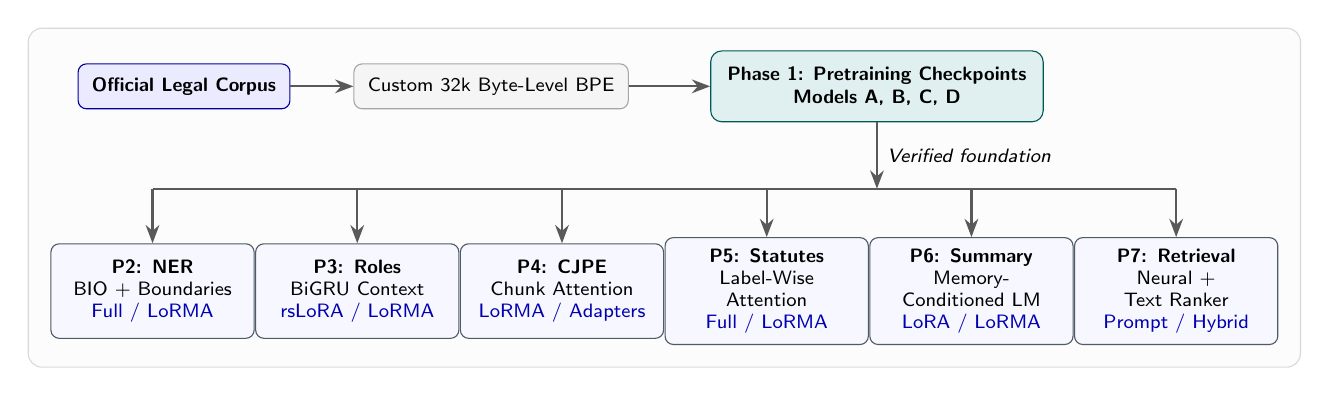
\begin{tikzpicture}[
font=\sffamily\small,>=Stealth,
data/.style={draw=blue!60!black,fill=blue!8,rounded corners=3pt,inner sep=5pt,align=center,font=\sffamily\scriptsize\bfseries},
proc/.style={draw=gray!70,fill=gray!8,rounded corners=3pt,inner sep=5pt,align=center,font=\sffamily\scriptsize},
phase1/.style={draw=teal!70!black,fill=teal!12,rounded corners=4pt,inner sep=6pt,align=center,font=\sffamily\scriptsize\bfseries},
task/.style={draw=slate!70!black,fill=blue!3!white,rounded corners=3pt,inner sep=4pt,align=center,text width=2.3cm,minimum height=1.2cm,font=\sffamily\scriptsize},
arrow/.style={->,thick,draw=gray!70!black}]
\node[data] (corpus) at (-4.8,2.6) {Official Legal Corpus};
\node[proc] (tok) at (-.9,2.6) {Custom 32k Byte-Level BPE};
\node[phase1] (p1) at (4.0,2.6) {Phase 1: Pretraining Checkpoints\\Models A, B, C, D};
\draw[arrow] (corpus)--(tok);\draw[arrow] (tok)--(p1);
\coordinate (split) at (4,1.3);
\draw[arrow] (p1.south)--(split) node[midway,right,font=\sffamily\scriptsize\itshape] {Verified foundation};
\node[task] (p2) at (-5.2,0) {\textbf{P2: NER}\\BIO + Boundaries\\\textcolor{blue!70!black}{Full / LoRMA}};
\node[task] (p3) at (-2.6,0) {\textbf{P3: Roles}\\BiGRU Context\\\textcolor{blue!70!black}{rsLoRA / LoRMA}};
\node[task] (p4) at (0,0) {\textbf{P4: CJPE}\\Chunk Attention\\\textcolor{blue!70!black}{LoRMA / Adapters}};
\node[task] (p5) at (2.6,0) {\textbf{P5: Statutes}\\Label-Wise Attention\\\textcolor{blue!70!black}{Full / LoRMA}};
\node[task] (p6) at (5.2,0) {\textbf{P6: Summary}\\Memory-Conditioned LM\\\textcolor{blue!70!black}{LoRA / LoRMA}};
\node[task] (p7) at (7.8,0) {\textbf{P7: Retrieval}\\Neural + Text Ranker\\\textcolor{blue!70!black}{Prompt / Hybrid}};
\draw[thick,gray!70!black] (p2.north|-split)--(p7.north|-split);
\foreach \p in {p2,p3,p4,p5,p6,p7}{\draw[arrow] (\p.north|-split)--(\p.north);}
\begin{scope}[on background layer]
\node[draw=gray!30,fill=gray!2,rounded corners=5pt,inner sep=8pt,fit=(corpus)(p1)(p2)(p7)] {};
\end{scope}
\end{tikzpicture}}
\caption{Six task-specific descendants derived from the own Phase-1 checkpoints, with task-specific adaptation and inference.}
\label{fig:arch_flow}\end{figure*}

Full fine-tuning updates the backbone and head; partial fine-tuning exposes selected
upper blocks/norms. LoRA uses $W_{\rm eff}=W_0+(\alpha/r)BA$ ;
rsLoRA replaces $r$ with $\sqrt r$ . The implemented
identity-inflated multiplicative residual follows
\begin{equation}
W_{\rm eff}=(I+sBA)W_0,\qquad s=\alpha/r,
\end{equation}
with the original bias outside the update. This is matrix multiplication, not
$W_0\odot(1+BA)$; it is a LoRMA-style implementation \cite{bihany2025lorma}.
Bottleneck adapters add residual down/up projections .
BitFit exposes biases and, in this implementation, selected norm parameters
. IA3 learns activation scales . Prompt tuning
learns input embeddings; prefix tuning inserts learned attention keys/values
.

Classification KD combines supervised loss with temperature-scaled teacher matching
, typically $T^2D_{\rm KL}(p_T\|p_S)$, rather than
silently reversing the KL arguments. Multi-label and sequence tasks require their
own matching losses. A completed own task teacher, not an observation ZIP alone,
must supply the teacher signal.

\subsection{Phase 2 - Legal NER}
Token and character features support 25 BIO classes for 12 entity types. Learned
boundary heads, document-level evidence fusion and constrained BIO Viterbi decoding
recover consistent entity spans across overlapping windows. Validation calibration
balances precision and recall. The implemented methods are A full, B LoRA, C adapters,
D partial, A LoRMA and B distillation. B supplies bidirectional encoder features;
all predicted spans retain the original exclusive-end character offsets.

\subsection{Phase 3 - Rhetorical role prediction}
Mean/last token-piece features are pooled to sentences, combined with domain and
position features, and processed by a document-level bidirectional GRU before a
13-way classifier. The context layer is not a bidirectional Transformer. Experiments
use A LoRMA, A rsLoRA, B LoRA, C IA3, D prompts and B distillation. Supplied sentence
order is retained. Sentence-only and higher-dropout runs test context and regularization
but do not constitute new adaptation methods.

\subsection{Phase 4 - Court judgment prediction}
Chunk mean/last features are projected, augmented with position features and aggregated
using recurrent context and attention pooling. Binary logits are calibrated on dev.
The method implementations comprise A full, A LoRMA, B BitFit, C adapters, D partial
and B distillation. A LoRMA is the selected competition system, with reported
Macro-F1 0.7705 and rank 31.

\subsection{Phase 5 - Legal statute identification}
Independent sigmoid probabilities predict the 100 statute labels. Shared document
features and label-specific evidence attention support positive-weighted BCE, with
asymmetric loss available as an option. The saved selected full-tuning configuration
uses BCE. Calibration compares raw, global and shrunk per-label decisions. The method
implementations are A full, A LoRMA, B prompts, C adapters, D partial and B distillation.
A full is the selected competition system, with reported Macro-F1 0.3970.

\subsection{Phase 6 - Abstractive summarization}
Pooled source-chunk vectors form learned, position-aware, salience-weighted document
memory. A/C/D use this as a causal prefix in their own blocks; B uses encoder--decoder
cross-attention. Teacher-forced target windows retain context and cover the complete
target. Methods are A LoRMA, A LoRA, B encoder/decoder prompts, C Houlsby adapters,
D Pfeiffer adapters and smaller-B sequence distillation. The executed KD output now
contains a verified student submission and four completed epochs.
\begin{equation}
\mathcal L_{\rm seqKD}=0.75\mathcal L(y_{\rm gold})+0.25\mathcal L(y_{\rm teacher}).
\end{equation}
A completed larger own teacher generates Train-only targets internally on both GPUs,
with durable per-document journals. B remains an encoder--decoder, not a causal-only
student. The saved decoding rule is greedy with maximum 512 tokens, minimum 32,
repetition penalty 1.1 and blocked three-grams; a beam-four result is not evidenced.
The reported KD/teacher score ratio is about 98.6\%, but a ratio of BERTScores is
not a percentage of retained legal capability. Saved total parameter counts provide
a more concrete size comparison: about 113.2M for A LoRA versus 62.8M for B KD.
This does not establish an equivalent runtime-memory reduction.

\subsection{Phase 7 - Prior Case Retrieval (PCR)}
Verified frozen lower-layer memories encode the complete source. Adapted upper layers
and separate query and candidate projections remain live during contrastive training.
The implemented adaptation methods are A LoRMA, A partial, B prompts, C IA3, D K/V
prefixes and B distillation. The selected B prompt model combines its neural signal
with a learned official-text ranking layer.

Dense and BM25  rankings are combined by a tune-selected
weighted reciprocal-rank rule \cite{cormack2009rrf}:
\begin{equation}
s(d)=\frac{w}{k+r_{\rm neural}(d)}+\frac{1-w}{k+r_{\rm BM25}(d)}.
\end{equation}
A later ranking stage trains a histogram gradient-boosted classifier from scratch
on all official training query--candidate pairs. Features combine lexical, section,
passage and public citation evidence; candidate IDs are not used as predictive features.
The tuned rule combines learned text ranking with the own neural ranking. For B prompts,
the saved enhanced output uses neural weight 0.1 and rank constant 20. It reports
dev Micro-F1@7 0.472485, tune 0.491143 and confirmation 0.430880. The final reported
competition score is 0.4365. This stage complements the adapted encoder and is not
counted as an additional PEFT method.

\section{Experiments and Implementation Details}
\subsection{Compute and training protocol}
Kaggle T4 $\times2$ is the training target. Importable modules are materialized from
notebook cells before \texttt{mp.spawn} starts two NCCL DDP workers. The implementation
uses FP16 autocast, dynamic loss scaling, gradient clipping, AdamW and warmup/decay
schedules, with rank-0 progress bars. The recurrent components use stable precision
paths where required. Multiple GPU processes allow parallel computation but do not
guarantee full device utilization at every stage.

Early C/D runs exposed long execution times relative to the available session budget.
Architecture-specific token caches and full-state recovery made multi-session training
manageable. Atomic checkpoints preserve model weights, optimizer moments, scaler,
scheduler, epoch, step, next-batch cursor and per-rank RNG state. Two recovery slots
and validation-best receipts are saved every 500 updates and at epoch boundaries,
allowing further epochs to continue the original optimization state.

Chunk microbatching, gradient accumulation and activation recomputation bound memory.
Later execution code uses pinned transfers, prefetch, equivalent short sparse masks,
frozen-prefix caching and batched generation. Frozen caches cannot replace adapted
layers during training. Summarization shares source memory across target windows;
the newer executor batches windows within a document and tunes safe microbatch caps.
These are execution improvements; no universal 3.5-fold speedup is claimed.

\begin{table}[H]\centering\small
\caption{Examples from saved winning-method configurations, not guessed cross-phase defaults.}
\begin{tabular}{llrrl}\toprule
Run & Chunk/piece tokens & Backbone LR & Head/memory LR & Selected epoch\\\midrule
P3 A rsLoRA & 192 & 0.0002 & 0.0005 & 4\\
P4 A LoRMA & 256 & 0.0001 & 0.0002 & 4\\
P5 A full & 256 & 3e-05 & 0.0003 & 4\\
P6 A LoRA & 256 & 0.0002 & 0.0003 & 4 completed\\\bottomrule
\end{tabular}\end{table}
\subsection{Local evaluation}
NER holds out documents; RR/CJPE/LSI use their public dev views; summarization uses
grouped train/tune/confirmation. Retrieval divides official dev into tune and confirmation.
Dev-selected calibration is labelled as fitted evidence, not an independent test
estimate. Checkpoint/source/tokenizer manifests and strict ID/schema checks protect
provenance and packaging. They cannot rule out memorization or certify legal accuracy.

\subsection{Ablations and controlled comparisons}
The RR sentence-only run gives local F1 0.362606, compared with 0.429851 for contextual
rsLoRA: a 0.067245 difference in those saved runs. The LoRMA dropout trial gives
0.429916 versus 0.437545 in the original. These single-run comparisons support further
testing, not a multi-seed causal claim. In NER, the calibrated ensemble's reported
0.4839 does not exceed A full's 0.4851. For retrieval, A LoRMA's dense tune score
0.233494 and fused tune score 0.301127 are a same-split comparison; the frozen fused
confirmation score is 0.240575.

\section{Results}
Table~\ref{tab:variants} reports at least three competition variants per phase using
the primary score. Local evaluation and secondary metrics are summarized separately
so the competition comparison remains easy to read. The phase-specific metrics are
BERTScore for P1/P6, Macro-F1 for P2--P5 and Micro-F1@7 for P7.

\begingroup\scriptsize\setlength{\tabcolsep}{4pt}
\begin{longtable}{clrr}
\caption{Competition results for the reported variants. Score uses each phase's primary metric.}\label{tab:variants}\\
\toprule Phase & Variant & Score & Submission ID\\\midrule\endfirsthead
\toprule Phase & Variant (continued) & Score & Submission ID\\\midrule\endhead
1 & A (Causal Decoder) & 0.8348 & 958572 \\
1 & B (Enc-Dec Cross-Attn) & 0.7977 & 958564 \\
1 & C (Transformer-GRU Hybrid) & 0.8308 & 958568 \\
1 & D (Sparse-Attn Decoder) & 0.8264 & 960903 \\
2 & A Full FT & 0.4851 & 977344 \\
2 & A LoRMA  & 0.4839 & 977526 \\
2 & Validated Ensemble v1 & 0.4839 & 977669 \\
2 & D Partial FT & 0.4230 & 977521 \\
2 & C Bottleneck Adapters & 0.4072 & 977350 \\
2 & B LoRA  & 0.2019 & 977348 \\
2 & B Distillation (Teacher A) & 0.1438 & 977345 \\
3 & A rsLoRA  & 0.4560 & 993609 \\
3 & A LoRMA  & 0.4511 & 993608 \\
3 & C IA3  & 0.4185 & 993619 \\
3 & B Distillation (Teacher A) & 0.4106 & 993613 \\
3 & B LoRA  & 0.3843 & 993610 \\
3 & D Prompt Tuning & 0.4312 & 993612 \\
4 & A LoRMA FAST V2 & 0.7705 & 1009524 \\
4 & A Full FAST V2 & 0.7464 & 1009521 \\
4 & C Adapters FAST V2 & 0.7285 & 1009525 \\
4 & B Distillation FAST & 0.6294 & 1009526 \\
4 & B BitFit Bias Tuning & 0.5779 & 1007811 \\
5 & A Full FT & 0.3970 & 1013611 \\
5 & A LoRMA  & 0.3966 & 1013621 \\
5 & C Adapters Bottleneck & 0.3618 & 1013620 \\
5 & D Partial FT & 0.3850 & 1013608 \\
5 & B Prompt Tuning & 0.2783 & 1013618 \\
6 & A LoRA  & 0.8353 & 1043778 \\
6 & A LoRMA  & 0.8345 & 1043777 \\
6 & C Houlsby Adapters & 0.8277 & 1043780 \\
6 & B Sequence Distillation & 0.8237 & 1044525 \\
6 & D Pfeiffer Adapters & 0.8206 & 1043781 \\
6 & B Prompt Tuning & 0.8133 & 1043779 \\
7 & B Prompt + Hybrid RRF & 0.4365 & 1042346 \\
7 & A LoRMA + Hybrid RRF & 0.4353 & 1042349 \\
7 & B Distillation + RRF & 0.4353 & 1042352 \\
7 & A Partial FT + RRF & 0.4347 & 1042347 \\
7 & D Prefix Tuning + RRF & 0.4335 & 1042343 \\
7 & C IA3 + Hybrid RRF & 0.4330 & 1042344 \\
7 & A LoRMA Earlier hybrid export & 0.2676 & 1041957 \\
7 & A Partial Earlier hybrid export & 0.2623 & 1041958 \\
7 & B Prompt Earlier hybrid export & 0.2563 & 1041960 \\
7 & C IA3 Earlier hybrid export & 0.2493 & 1041961 \\
7 & D Prefix Earlier hybrid export & 0.2451 & 1041962 \\
\bottomrule\end{longtable}\endgroup
\begin{table}[htbp]\centering\scriptsize
\caption{Local evaluation snapshot. Values are Macro-F1 for P2--P5,
ROUGE-1/L pairs for P6, and dev Micro-F1@7 for P7. P4/P5 include selected
calibration; enhanced P7 includes the final text-ranking stage.}
\setlength{\tabcolsep}{3pt}
\begin{tabular}{llrllr}\toprule
Phase & Variant & Local metric(s) & Phase & Variant & Local metric(s)\\\midrule
P2 & A Full FT & 0.5347 & P5 & C Adapters & 0.3694 \\
P2 & A LoRMA & 0.5401 & P5 & D Partial FT & 0.3318 \\
P2 & D Partial FT & 0.4534 & P5 & B Prompt Tuning & 0.2850 \\
P2 & C  Adapters & 0.3593 & P6 & A LoRA & 0.4398/0.2141 \\
P2 & B LoRA & 0.1572 & P6 & A LoRMA & 0.4356/0.2118 \\
P2 & B Distillation (Teacher A) & 0.1425 & P6 & C Houlsby Adapters & 0.3716/0.1966 \\
P3 & A rsLoRA & 0.4299 & P6 & B Sequence Distillation & 0.3926/0.1981 \\
P3 & A LoRMA & 0.4375 & P6 & D Pfeiffer Adapters & 0.3621/0.1958 \\
P3 & C IA3 & 0.4196 & P6 & B Prompt Tuning & 0.3823/0.1985 \\
P3 & B Distillation (Teacher A) & 0.3584 & P7 & B Prompt + Hybrid RRF & 0.4725 \\
P3 & B LoRA & 0.4057 & P7 & A LoRMA + Hybrid RRF & 0.4714 \\
P3 & D Prompt Tuning & 0.3832 & P7 & A Partial FT + RRF & 0.4736 \\
P4 & A LoRMA FAST V2 & 0.7745 & P7 & D Prefix Tuning + RRF & 0.4703 \\
P4 & A Full FAST V2 & 0.7745 & P7 & C IA3 + Hybrid RRF & 0.4714 \\
P4 & C Adapters FAST V2 & 0.7626 & P7 & A LoRMA early hybrid & 0.2824 \\
P4 & B Distillation FAST & 0.6600 & P7 & A Partial early hybrid & 0.2879 \\
P4 & B BitFit Bias Tuning & 0.5948 & P7 & B Prompt early hybrid & 0.2702 \\
P5 & A Full FT & 0.4093 & P7 & C IA3 early hybrid & 0.2702 \\
P5 & A LoRMA & 0.4127 & P7 & D Prefix early hybrid & 0.2624 \\
\bottomrule\end{tabular}\end{table}


The strongest author-reported systems are A for Phases 1--6, with task-dependent
adaptation: full tuning for NER/statutes, rsLoRA for RR, LoRMA for CJPE and LoRA for
summarization. B prompt tuning leads reported retrieval. LoRMA is competitive, but
does not consistently beat full tuning: it is slightly below it in both NER and
statute prediction. These outcomes do not establish superiority under controlled
equal-compute conditions.

\begin{figure}[htbp]\centering
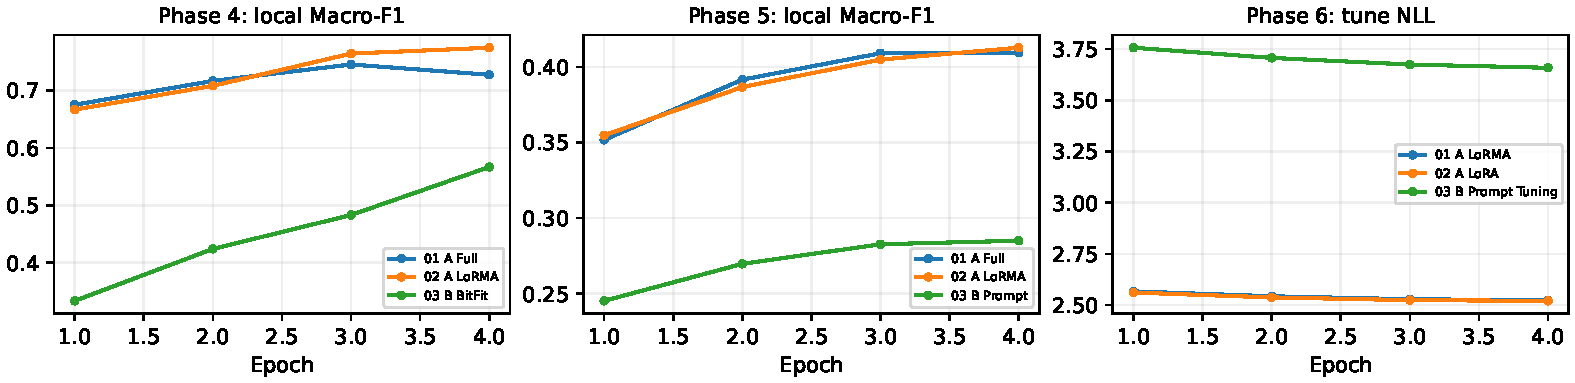
\includegraphics[width=\linewidth]{figures/saved_learning_curves.pdf}
\caption{Saved epoch histories track local F1 and tune NLL for the corresponding tasks.}
\end{figure}
\begin{figure}[htbp]\centering
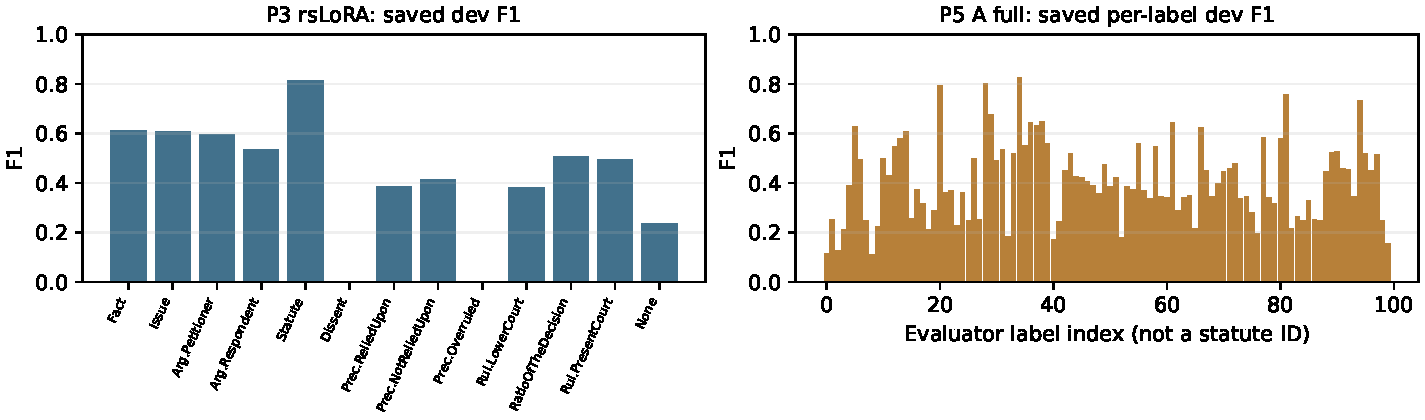
\includegraphics[width=\linewidth]{figures/per_label.pdf}
\caption{Saved per-label development scores. RR labels with zero gold support remain visible;
LSI uses evaluator label indices, not inferred statute names.}\label{fig:labels}
\end{figure}

In Phase 5, A full improves from raw dev Macro-F1 0.396887 to selected 0.409342,
with Micro-F1 0.499741. LoRMA has selected dev Macro-F1 0.412654 and Micro-F1
0.504139, yet the author reports a slightly lower private score than full tuning.
For P6 A LoRA, confirmation ROUGE-1/L are 0.439775/0.214084; B KD gives
0.392595/0.198119. BERTScore and ROUGE ordering need not coincide. The saved learning curves support direct inspection of training and validation dynamics.

\section{Error Analysis and Discussion}
\subsection{Phase-wise failure modes}
The Phase-1 audit motivated explicit repetition controls: 908 of 1,000 B continuations
exceeded its repeated-four-gram threshold. In NER, punctuation attached to citation
spans makes exact character reconstruction essential. Document-level fusion and BIO
constraints address inconsistent window predictions. RR's per-label diagnostics expose
weak classes that a single aggregate score can hide and guide attention to class support.

CJPE aggregation preserves terminal reasoning and outcome material alongside earlier
facts. Label-wise statute diagnostics guide threshold calibration and precision--recall
trade-offs. Summarization benefits from explicit length and repetition controls, while
legal faithfulness remains a useful focus for qualitative evaluation. Retrieval combines
semantic and official-text evidence to connect legal terminology with learned relevance.

A useful retrieval comparison comes from the executed final ranking stage: B prompt
baseline dev Micro-F1@7 is 0.270150, compared with enhanced dev 0.472485 after the
official-text learner and tuned fusion. Its independent confirmation value is 0.430880.
These measurements demonstrate the practical contribution of the complete ranking
pipeline, while keeping tune selection and confirmation evidence separate.

\subsection{What the metrics do not measure}
Exact-span F1 jointly tests boundaries and labels. Macro-F1 can be sensitive to very
small class support. Micro-F1@7 evaluates against the complete gold relevance set,
including queries with more or fewer than seven relevant cases. BERTScore and ROUGE
measure similarity to reference wording or representations; neither verifies that
a generated holding is legally correct. The models are benchmark systems, not
validated legal advisers.

\subsection{Limitations and what I would do next}
The next steps build on the established pipeline: longer own-model pretraining,
structural transfer from NER/RR into judgment prediction, and lightweight cross-encoder
reranking on official hard negatives. Matched split, tokenizer, source-budget and
update-count comparisons can strengthen conclusions about each component. Separate
confirmation data and legal faithfulness review provide a clear route toward more
reliable deployment.

\subsection{Surprising findings}
The experiments show that compact adaptation can be competitive with full tuning,
while task-specific calibration and ranking provide useful additional leverage.
In statute prediction, the stronger calibrated local score does not automatically
determine the best competition score. This makes the combination of careful local
evaluation, confirmed submission records and reproducible execution especially valuable.

\section{Conclusion}
The project connects scratch legal-language modelling to six downstream tasks using
four own foundations and multiple adaptation strategies. Bounded-memory preprocessing,
exact offset reconstruction, hierarchical document encoding and resumable dual-GPU
training make the system practical under Kaggle constraints. The reported results
show the value of choosing adaptation and inference for each task rather than relying
on model size alone. The final source bundle preserves the selected implementations
and their configurations, providing a clear basis for reproduction and further work.

\clearpage
\section*{LLM Usage Declaration}
% ============================================================
This declaration records the assistance used in the project and report.
\medskip
\noindent
\textbf{Q1.} Which Large Language Model(s), if any, did you use while completing the competition or writing this report? Give model name and vendor (e.g., none / ChatGPT-4.x / Gemini~x / Claude~x / Grok / Copilot / other). \\[0.6em]
Answer: OpenAI ChatGPT/Codex (OpenAI).
\medskip
\noindent
\textbf{Q2.} For each row, mark Yes or No and state the purpose in one short phrase. ``Yes'' is acceptable only for the uses permitted by the capstone document.
\begin{table}[H]
\centering
\begin{tabular}{>{\raggedright\arraybackslash}p{4.6cm}|c|>{\raggedright\arraybackslash}p{7.2cm}}
\toprule
Part & Used LLM? & Purpose of using the LLM \\
\midrule
Understanding concepts / papers & Yes & Explanations of architectures and adaptation methods. \\
Ideation / brainstorming at a high level & Yes & Experiment planning and suggested approaches. \\
Debugging small ancillary snippets & Yes & Path, syntax and checkpoint compatibility debugging. \\
Plotting / visualization code & Yes & Report plots and artifact inspection. \\
Grammar / writing style of the report & Yes & Editing the supplied prose. \\
Report structure / section wording & Yes & LaTeX organization and template checks. \\
Designing the model architecture & Yes & Assistance implementing prescribed model families and task heads. \\
Hyperparameter search / tuning & Yes & Proposed training settings and experiment plans. \\
Analysis of results / conclusions & Yes & Earlier interpretation of results; author supplied updated findings. \\
Writing the core training / inference code & Yes & Substantial generated and revised notebooks. \\
Other (specify) & Yes & GPU optimization, evaluation and packaging assistance. \\
\bottomrule
\end{tabular}
\end{table}
\medskip
\noindent
\textbf{Q3.} Did you refer to sources other than lecture slides and an LLM?
If yes, list them (papers, blogs, GitHub repositories, textbooks, official starter notebook, evaluation scripts). These must also appear in the bibliography when they influenced the method. \\[0.4em]
Answer: Official course materials, starter/evaluation code and the key papers cited below. Full method references are documented in the accompanying code bibliography.
\medskip
\noindent
\clearpage\noindent\textbf{Q4.} Apart from any permitted LLM use, what was \emph{your} contribution? In 8--12 sentences describe your own understanding, architecture decisions, implementation, experiments, and analysis. Name at least two things you tried that failed and what you concluded from them.
\medskip
\noindent

\noindent I ran and organized experiments across all seven phases on Kaggle.
I attached the appropriate data, tokenizer and model outputs and managed saved versions.
I monitored scores and requested changes when runs failed or performance was low.
Long C/D runs and session limits led me to use recoverable checkpoints and different token budgets.
Independent NER window predictions exposed boundary errors, prompting document-level decoding checks.
I compared adaptation methods and recorded the negative results of extra calibration and ensembling.
I preserved executed notebooks and artifacts to make the experiments reviewable.
I supplied the final competition results, research questions and proposed next experiments used in this report.
ChatGPT/Codex supplied substantial implementation, debugging and planning assistance, which I have disclosed above.
I remain responsible for checking the submitted results, understanding the implementation and explaining its limitations.


\clearpage
\bibliographystyle{ieeetr}\bibliography{references}
\end{document}
